% methodology_v1.tex -- the reformatted Method, drafted 2026-09-08 on Sinem's
% comments. It follows the shape of CURE (PoPETs 2026): an unnumbered lead of
% Problem Statement, Threat Model and Motivation, then a named Overview, then
% numbered subsections whose third-level headings name their content.
%
% NOT in the build. sections/method.tex is still what main.tex and main-tr.tex
% input. Compile this one through main-v1.tex.
%
% Differences from method.tex, all deliberate:
%   - the C1 to C6 list is dissolved into the Motivation prose
%   - \paragraph run-ins become \subsubsection, so they number rather than letter
%   - every run-in is renamed to name its content
%   - the ten semicolons are gone
%   - the protocol is called "the protocol", not HE-OFT
%   - Method points at fig:training, which still lives in the introduction

\section{Method}
\label{sec:method}
\label{sec:setting}

\paragraph{Problem Statement} We consider $\Nc$ clients holding private labeled
data over a common label space of $\Cc$ classes. Client $j$ holds data $\Dj$ of
size $\nj$. The class proportions differ across clients, and a client may hold no
example of a class. The clients seek a classifier that operates across the entire
label space, and they cannot pool their data to train a single model. Three
requirements separate this setting from vanilla federated learning. The protocol
is \emph{one-shot}, and each client uploads its encrypted head displacement once.
Confidentiality rests on cryptography, and a client's contribution is never
available in plaintext to any other party. The trained classifier is never
disclosed, and no party, client or server, ever holds it in plaintext.

\paragraph{Threat Model} The participants are $\Nc$ clients and a server. A
static, semi-honest adversary corrupts the server together with up to $\tc-1$
clients. The corrupted parties follow the protocol, pool their views, and try to
infer private information from what they observe. \Cref{sec:security} states what
each party sees and proves the guarantees.

\paragraph{Motivation} \paperonly{Optimization cannot run under encryption at an
acceptable cost. All learning therefore happens in plaintext on the clients, and
the server performs no learning. Models trained from different starting points do
not combine linearly, and multiplicative depth dominates homomorphic cost. Every
client therefore starts from one public initializer on one frozen public
backbone, and the server combines what it receives by a linear combination.

Intermediate training signals are the strongest attack surface, as
\cref{sec:related-leakage} reports. The protocol is therefore one-shot, and its
single artifact is a ciphertext. No single party may decrypt that artifact. The
secret key is generated and held distributively under multiparty CKKS
(\cref{sec:mhe}).

The model is never disclosed, yet it must answer queries. The client that asks a
query computes the features of that query itself. It therefore runs the backbone
and its own adapter in plaintext, and the shared trained quantity cannot sit
inside the backbone. A server computing on ciphertexts cannot inspect a value or
compare two of them, hence it cannot apply an aggregation rule that depends on
the data. The clients make that choice instead (\cref{sec:selection}).}

\tronly{Optimization cannot run under encryption at an acceptable
cost. Gradient steps, softmax, and adaptive curvature need deep circuits that
bootstrap repeatedly. All learning therefore happens in plaintext on the clients,
and the server performs no learning. Models trained from different starting
points do not combine linearly, and multiplicative depth dominates homomorphic
cost. Every client therefore starts its trainable unit from one public
initializer on one frozen public backbone, and the server combines what it
receives by a linear combination. That is the cheapest operation the scheme
offers, and it is the only one the method needs.

Intermediate training signals are the strongest attack surface. Each exposed
round is a fresh training-time artifact, and \cref{sec:related-leakage} reports
what such artifacts give up. The protocol is therefore one-shot, and its single
artifact is a ciphertext. No single party may be able to decrypt that artifact.
The parties distrust one another and the server is semi-honest, so the secret key
is generated and held distributively under multiparty CKKS (\cref{sec:mhe}).

The model is never disclosed, yet it must answer queries. A query is formed from
features, and the client that asks the query computes those features itself. The
client therefore runs the backbone and its own adapter in plaintext, and the
trained quantity that is shared cannot sit inside the backbone. One further
choice follows from the same restriction on the server. A server that computes on
ciphertexts cannot inspect a value, compare two of them, or branch on the result,
so it cannot apply an aggregation rule that depends on the data. The clients make
that choice instead, without decrypting anything (\cref{sec:selection}).}

\subsection{Overview}
\label{sec:overview}

The protocol runs in two phases. In the first, each client fine-tunes an adapter
and a classifier head on the same frozen public backbone, keeps the adapter, and
uploads its head displacement once, weighted by its own per-class counts and
encrypted. \Cref{fig:training} shows that phase. In the second, a client computes
the features of its query itself, encrypts them, and sends them to the server,
which applies the encrypted head and reduces the encrypted logits to the index of
the largest. No party holds a key that opens the shared head alone.

\subsection{Shared Head Construction}
\label{sec:split}

\subsubsection{Local Training}
Each client uses the same frozen public backbone $\featx$, and trains a low-rank
adapter $A_j$ that adjusts the representation, and a classifier head $h_j$ on top
of it. Only the head is shared. Client $j$ encrypts the displacement $\disp = h_j
- \thz$ of its head from the public initializer and uploads it once. The server
combines the encrypted displacements into a single shared head and never decrypts
the result. The adapter is trained locally and never transmitted.

\subsubsection{Position of the Shared Map}
The client that sends an inference query must compute the features of that query
itself. If the shared trained quantity were an adapter placed inside the
backbone, the features would depend on it, and computing them would require
evaluating the backbone with encrypted weights. The client would then have to
evaluate every nonlinearity of the network homomorphically, which is the cost
this design exists to avoid. The trained quantity that is shared must therefore
attach after the last nonlinearity. In a transformer, the only such point is the
final linear map.

\paperonly{The requirement constrains the \emph{position} of the shared map, not
the task it serves. Any trained linear map placed after the final nonlinearity
satisfies this requirement, provided that the querying client can compute the
features fed into the map. A classifier head is one example. The vocabulary
projection in an autoregressive decoder is another. Placing the map earlier
forces the client either to evaluate the nonlinearities above it under encryption
or to decrypt an intermediate value, which hands back the numbers the serving
path withholds. We evaluate classification only.}

\tronly{The requirement constrains the \emph{position} of the shared map, not the
task it serves. Any trained linear map that comes after the last nonlinearity
satisfies it, provided the querying client can compute the features that enter
the map. A classifier head is one such map. The vocabulary projection of an
autoregressive decoder is another, since it is linear, comes after the final
layer normalization, and takes features the client can compute from a prefix it
generated itself. We evaluate classification only. The construction itself does
not depend on the label space being a set of classes, and \cref{sec:scope}
records what a generation setting would additionally require, including the
restriction to greedy decoding that \cref{sec:serving} imposes.}

The adapter is relocated. Each client retains its own, thus the representation
still adapts to local data. The distinction follows from coverage. A client can
improve its own representation alone, but it cannot learn to recognize a class it
has never observed. Coverage is a property of the head, which is exactly what the
federation supplies. \Cref{sec:exp-split} measures both halves.

Retaining the adapter locally has a second consequence, which is cryptographic.
No aggregate of the adapters is ever formed. \Cref{sec:threat} states this
precisely.

\subsubsection{Coverage-Weighted Merge}
Let $g_{j}\in\mathbb{R}^{\Cc}$ collect client $j$'s per-class example counts,
$g_{j,c}=n_{j,c}$. The shared head is the coverage-weighted combination
\begin{equation}
\label{eq:aggregate}
\thstar \;=\; \thz \;+\; \frac{\sum_{j=1}^{\Nc} g_j \odot \disp}
                              {\sum_{j=1}^{\Nc} g_j},
\end{equation}
in which row $c$ of the shared head is the count-weighted average of the clients'
row-$c$ displacements. Clients holding a class decide its row, and rows that no
client covers remain at the public initializer. Each client forms the products
$g_j\odot\disp$ locally, before encryption, thus the server only adds
ciphertexts.

\subsubsection{Division by the Class Totals}
The denominator of \cref{eq:aggregate} is the vector of federation-wide per-class
totals. It cannot be decrypted. Every client knows its own counts, hence a
coalition of $\Nc-1$ clients that learned the totals would subtract its own and
read the remaining client's class histogram exactly. The reciprocal is therefore
evaluated under encryption, using an inversion circuit over the positive domain
whose refreshes are collective. It is paid once, at aggregation, never per query.

\tronly{\begin{algorithm}[t]
\caption{Building the shared head. All clients hold the same frozen public
backbone $\featx$ and the same public head initializer $\thz$.}
\label{alg:train}
\small
\begin{algorithmic}[1]
\State clients run distributed key generation, obtaining a collective public key
\For{client $j=1,\dots,\Nc$ \textbf{in parallel}}
  \State train adapter $A_j$ and head $h_j$ on $\Dj$ \Comment{plaintext, local}
  \State \textbf{keep} $A_j$, which is never transmitted
  \State send $\mathsf{Enc}(g_j\odot\disp)$ and $\mathsf{Enc}(g_j)$,
         where $\disp=h_j-\thz$
\EndFor
\State \textbf{server} adds the ciphertexts to form the numerator and the
       denominator of \cref{eq:aggregate} \Comment{additions only}
\State \textbf{server} evaluates the reciprocal of the denominator under
       encryption and multiplies \Comment{once, not per query}
\State \Return $\mathsf{Enc}(\thstar)$, which no party decrypts
\end{algorithmic}
\end{algorithm}}

\subsubsection{Aggregation Cost}
The server performs one ciphertext addition per client per ciphertext, one
encrypted reciprocal, and one multiplication. The encrypted object is the head
alone, whose size is set by the number of classes and the feature dimension.
Communication is one upload per client and no download of model parameters at
all.

\subsection{Encrypted Inference}
\label{sec:serving}

\tronly{\begin{figure*}[t]
\centering
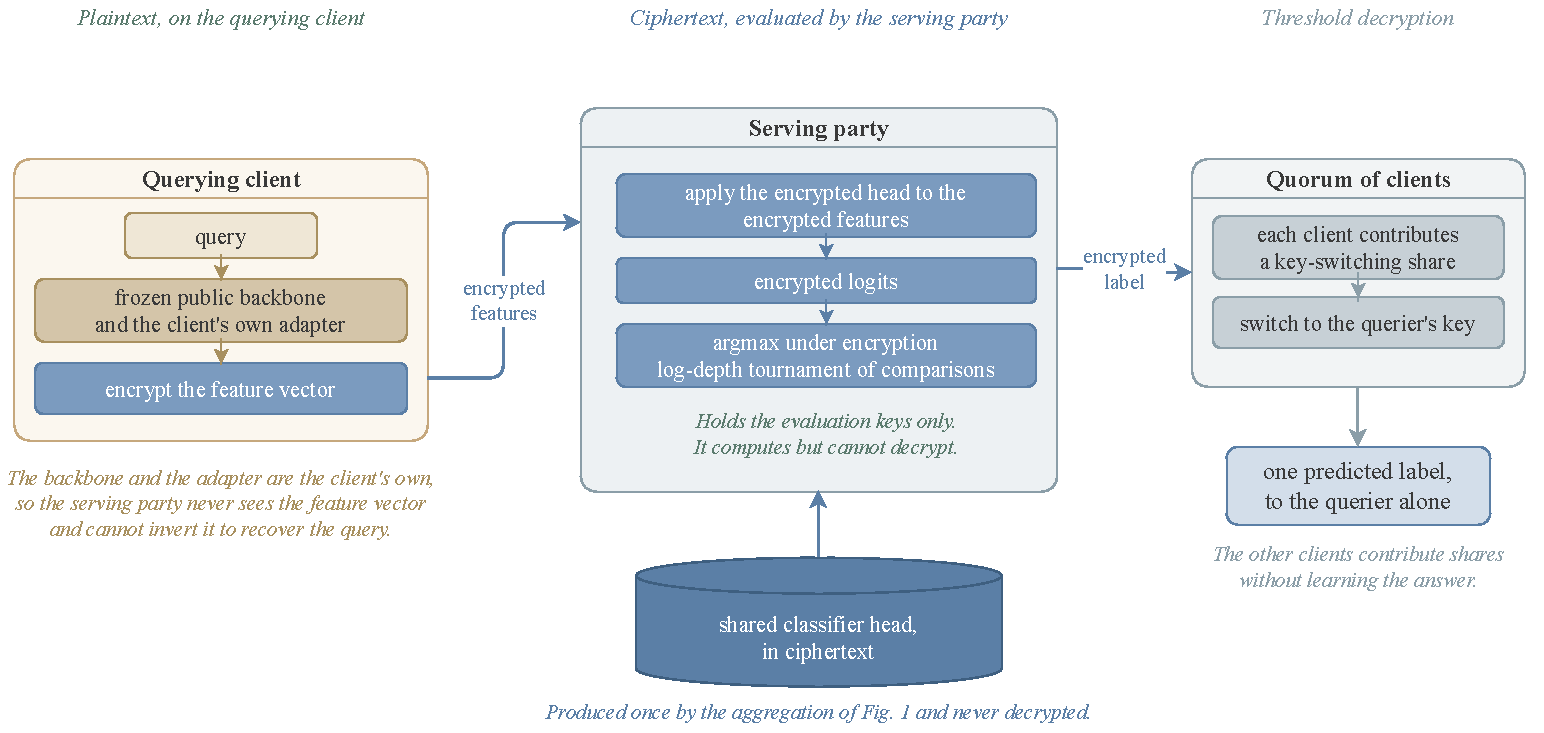
\includegraphics[width=\textwidth]{figures/fig_serving.pdf}
\caption{Answering one query. The querying client computes the features with its own backbone and adapter and encrypts them, so the server never sees the feature vector and cannot invert it to recover the query. The server holds the evaluation keys only. It applies the encrypted head, obtains encrypted logits, and reduces them to the index of the largest entry by a tournament of homomorphic comparisons. A quorum of clients then switches that index to the querying client's key, so the other clients contribute shares without learning the answer.}
\label{fig:serving}
\end{figure*}
}

\paperonly{The construction below serves a trained quantity that is linear in the
features. Serving a trained quantity that sits inside the backbone is the problem
that secure transformer inference addresses. An encrypted shared adapter composes
with those systems at the cost they report, and we place that case outside our
scope.}

\tronly{The construction below serves a trained quantity that is linear in the
features. Serving a trained quantity that sits inside the backbone is the problem
that secure transformer inference addresses. An encrypted shared adapter composes
with those systems at the cost they report, and we place that case outside our
scope. One difference should be noted. Those systems evaluate a plaintext model
on encrypted inputs, whereas here the shared weights are encrypted as well, so
each adapter site would carry a ciphertext-by-ciphertext product. The dominant
cost in that literature is the nonlinearities, which are unchanged, thus the
added cost is the low-rank product per site rather than a different order of
magnitude.}

\subsubsection{Query Serving}
A client that wants a prediction computes the features of its query with its own
backbone and adapter, encrypts them, and sends the ciphertext to the server. The
server applies the encrypted shared head to the encrypted features, obtains
encrypted logits, and reduces them to the index of the largest entry under
encryption. \Cref{alg:serve} states it.

\subsubsection{Query Encryption}
\paperonly{The client could send the features in plaintext, which would make the
head application cheaper. We encrypt them because features are invertible. A
party holding $\varphi_j(x)$ and the public backbone can reconstruct an
approximation of $x$. Sending features in plaintext would therefore hand the
server the client's input, which is the thing the protocol exists to protect.}

\tronly{The client could send the features in plaintext, which would make the
head application cheaper. We encrypt them because features are invertible. A
party holding $\varphi_j(x)$ and the public backbone can reconstruct an
approximation of $x$. Sending features in plaintext would therefore hand the
server the client's input, which is the thing the protocol exists to protect. The
price is that the server applies the head ciphertext by ciphertext rather than
ciphertext by plaintext, and \cref{sec:exp-cost} reports what that costs.}

\subsubsection{Label-Only Output}
\paperonly{Returning logits would defeat the construction. The head is a linear
map on features the client computes itself, therefore a client that reads logits
for feature vectors of its choosing recovers the head by solving a linear system
in as many queries as the feature dimension~\cite{tramer2016stealing}. The same
object, the final projection layer of a production transformer, has been
recovered through a deployed interface for a few tens of
dollars~\cite{carlini2024stealing}. Returning only the index of the largest entry
places an adversary in the hard-label setting, where functionally equivalent
extraction is markedly harder~\cite{chen2024hardlabel}. It does not make
extraction impossible, and \cref{sec:threat} states the resulting bound as a
bound on queries.}

\tronly{Returning logits would defeat the construction. The head is a linear map
on features the client computes itself, therefore a client that reads logits for
feature vectors of its choosing recovers the head by solving a linear system in
as many queries as the feature dimension~\cite{tramer2016stealing}. This is not a
hypothetical concern. The same object, the final projection layer of a production
transformer, has been recovered through a deployed interface for a few tens of
dollars, using an interface that exposed log-probabilities and a logit bias, and
the operators' response was to restrict that combination~\cite{carlini2024stealing}.
Returning only the index of the largest entry is the same restriction imposed by
construction rather than by policy. It places an adversary in the hard-label
setting, where functionally equivalent extraction has only recently been achieved
for general networks~\cite{chen2024hardlabel,carlini2025hardlabel}. Those results
carry a factor exponential in the number of hidden neurons, and our shared
quantity has none, thus the restriction buys less here than they suggest. It
removes the linear solve and puts a search for decision boundaries in its place,
at a factor logarithmic in the precision demanded, and it leaves the head
determined only up to a positive scale and a vector added to every row. It does
not make extraction impossible, and \cref{sec:threat} states the resulting bound
as a bound on queries rather than a cryptographic hardness claim.}

\subsubsection{Decryption to the Querier}
Decryption needs a quorum, and clients other than the querier take part in
answering each query. They contribute partial decryptions and read nothing,
because the quorum key-switches the ciphertext to the querying client's public
key rather than decrypting the label collectively.

\begin{algorithm}[t]
\caption{Answering one query. The shared head remains a ciphertext throughout.}
\label{alg:serve}
\small
\begin{algorithmic}[1]
\Require query $x$ at client $j$; $\mathsf{Enc}(\thstar)$ held by the server
\State client $j$ computes $\varphi_j(x)$ with its own backbone and adapter
       \Comment{plaintext, local}
\State client $j$ sends $\mathsf{Enc}(\varphi_j(x))$
\State \textbf{server} computes
       $\mathsf{Enc}(\ell) \gets \mathsf{Enc}(\thstar)\,\mathsf{Enc}(\varphi_j(x))$
       \Comment{ciphertext by ciphertext}
\State \textbf{server} reduces $\mathsf{Enc}(\ell)$ to
       $\mathsf{Enc}(\hat{y})$, $\hat y=\arg\max_c \ell_c$, by a tournament of
       homomorphic comparisons~\cite{cheon2020comparison}
\State a quorum of clients key-switches $\mathsf{Enc}(\hat y)$ to client $j$'s
       public key
\State \Return $\hat y$, readable by client $j$ alone
\end{algorithmic}
\end{algorithm}

\subsubsection{Serving Cost}
\paperonly{The argmax is the one operation in the protocol that costs more than
one level, because it compares logits rather than adding or scaling them. Packing
the logits into one ciphertext and reducing them by a tournament lowers the
number of sequential comparisons from $\Cc-1$ to $\lceil\log_2\Cc\rceil$, and
\cref{sec:exp-cost} reports the measured result. The server is not trusted with
anything. It holds the collective public key, the evaluation keys, and
ciphertexts, so it computes but cannot decrypt.}

\tronly{The argmax is the one operation in the protocol that costs more than one
level, because it compares logits rather than adding or scaling them. Evaluated
as a sequential fold of $\Cc-1$ comparisons, it costs minutes for a large label
space. Packing the logits into one ciphertext and reducing them by a tournament
lowers the number of sequential comparisons from $\Cc-1$ to
$\lceil\log_2\Cc\rceil$, and \cref{sec:exp-cost} reports the measured result.
None of this is particular to the multiparty setting. Homomorphic evaluation
under a collectively generated key is identical to evaluation under a single key,
and the schemes differ only in key generation and in decryption, therefore
single-key results carry over. The server is not trusted with anything. It holds
the collective public key, the evaluation keys, and ciphertexts, so it computes
but cannot decrypt, and it learns neither the model nor any client's data. It is
trusted only for availability, and where honest computation must be certified,
verifiable homomorphic encryption applies~\cite{viand2023verifiable}.}

\subsection{Arrangement Selection}
\label{sec:selection}

\tronly{\begin{figure*}[t]
\centering

\includegraphics[width=\textwidth]{figures/fig_selection.pdf}
\caption{Choosing between two arrangements without decrypting either. Each client scores both on data held back from its own training, selecting the logit of the true class with a plaintext mask, which is public because the client knows its own labels. The per-class counts are weighted by each class's share of the federation's examples, taken from the count matrix already used for the aggregation. The shared arrangement pools evidence across clients because it is one model; the personal arrangement cannot, and classes a client does not hold contribute nothing, which makes its score a lower bound. Exactly one value is decrypted.}
\label{fig:selection}
\end{figure*}
}

\subsubsection{Encrypted Scoring}
Two arrangements are available at the same cost: the shared head over each
client's own adapter, and the shared head over the bare public backbone with no
adapter at all. Which is better depends on the task, and the federation must
choose without decrypting either. Each client evaluates both on data it holds
back from its own training, entirely under encryption, and reports encrypted
per-class counts. The server combines the counts into one encrypted score per
arrangement, and the federation decrypts exactly one value, the index of the
arrangement it adopts.

\subsubsection{Prior-Weighted Estimator}
Each client could instead measure both arrangements on its held-out data and
vote. That procedure estimates the wrong quantity, and \cref{sec:exp-select}
shows it choosing wrongly whenever the two arrangements differ.
Score both arrangements as the expected accuracy of a prediction on an example
drawn from the federation's own class distribution,
\begin{equation}
\label{eq:estimator}
E \;=\; \sum_{c=1}^{\Cc} p_c\,a_c,
\qquad
p_c \;=\; \frac{\sum_j n_{j,c}}{\sum_j \nj},
\end{equation}
where $a_c$ is the accuracy on class $c$ and $p_c$ is that class's share of the
federation's examples, taken from the per-class counts already used in
\cref{eq:aggregate}. For the shared arrangement, there is one model, hence
per-class evidence from different clients concerns the same object and combines.
For the personal arrangement each client's evidence concerns only its own model,
and classes it does not hold contribute no evidence at all. Scoring those classes
at zero makes $E$ a lower bound for the personal arrangement. There is no fitted
threshold anywhere.

\tronly{\begin{algorithm}[t]
\caption{Choosing an arrangement without decrypting either. Nothing is revealed
except the index of the winner.}
\label{alg:select}
\small
\begin{algorithmic}[1]
\For{each arrangement $m$ and each client $j$}
  \For{each held-out example $(x,y)$ of client $j$}
    \State obtain $\mathsf{Enc}(\ell)$ and $\mathsf{Enc}(\max_c \ell_c)$ as in
           \cref{alg:serve}
    \State select $\mathsf{Enc}(\ell_{y})$ with a plaintext mask
           \Comment{the client knows $y$, thus the mask is public}
    \State add $\mathsf{Enc}\big(\mathbf{1}[\ell_y = \max_c \ell_c]\big)$ to the
           class-$y$ accumulator
  \EndFor
\EndFor
\State combine the accumulators into $\mathsf{Enc}(E_m)$ by \cref{eq:estimator},
       using public scalars \Comment{depth one}
\State compare the two encrypted scores
\State \Return the decrypted index of the larger \Comment{one value}
\end{algorithmic}
\end{algorithm}}

\subsubsection{One Example per Class}
\paperonly{The estimator needs an estimate of accuracy on classes a client has
not seen, and its only local proxy is accuracy on classes it has barely seen.
Each client therefore reserves at least one held-out example from every class it
holds before carving the remainder at random. This costs a negligible amount of
training data and requires no change to the cryptographic protocol.}

\tronly{The estimator needs an estimate of accuracy on classes a client has not
seen, and its only local proxy is accuracy on classes it has barely seen. A
held-out set carved uniformly almost never contains a class the client holds one
or two examples of, thus that proxy is unmeasurable. Each client therefore
reserves at least one held-out example from every class it holds before carving
the remainder at random. A client holding a single example of a class donates it,
thus its adapter never trains on that class, which is exactly the probe the
estimator needs. This costs a negligible amount of training data and requires no
change to the cryptographic protocol.}

\subsubsection{Cost and Disclosure}
Every step is depth one except the comparisons, which are the same circuit
already used for the argmax. One value is decrypted for the whole federation. The
per-client per-class accuracies are not decrypted, and must not be.
